%!TEX TS-program = xelatex
%!TEX encoding = UTF-8 Unicode
\documentclass[17pt]{memoir}

\usepackage{xltxtra,fontspec,xunicode}
\defaultfontfeatures{Scale=MatchLowercase}
%\setromanfont[Numbers=Uppercase]{Hoefler Text}
%\setmonofont[Scale=0.90,Ligatures=NoCommon]{Courier}

\setmainfont{CMU Sans Serif}
%\setmainfont[BoldFont={OpenDyslexic3-Bold.ttf} ]{OpenDyslexic3-Regular.ttf}
%\setmainfont[
% BoldFont={OpenDyslexic-Bold.otf}, 
% ItalicFont={OpenDyslexic-Italic.otf},
% BoldItalicFont={OpenDyslexic-BoldItalic.otf}
% ]{OpenDyslexic-Regular.otf}

%\usepackage{natbib}

\usepackage{hyperref}
\hypersetup{
    colorlinks=true,       % false: boxed links; true: colored links
    linkcolor=black,          % color of internal links (change box color with linkbordercolor)
    citecolor=black,        % color of links to bibliography
    filecolor=blue,      % color of file links
    urlcolor=blue           % color of external links
}

\title{Dyslexia}
\author{Lyron Winderbaum}

\begin{document}

\maketitle



Dyslexia is estimated to occur in 15-20\% of the Australian population, around 10\% being diagnosed with dyslexia and the rest being undiagnosed. Under the conservative assumption that only 10\% of students have dyslexia, any given class of 25 randomly selected students will have \textbf{at least 2 students} with dyslexia with a probability over 70\%. In the more realistic case that 20\% of students have dyslexia, as claimed by the \href{https://dyslexiaassociation.org.au/dyslexia-in-australia/}{Australian Dyslexia Association}, this probability rises to over 97\%. Taking into account the possibility for undiagnosed dyslexia (particularly for students who went through primary school in another country, and students whose dyslexia might be masked by another learning disability), the conclusion is that it is reasonable to conduct ourselves as teachers under the assumption that every one of our classes will have dyslexic students in them, if we have identified them or not. 

Knowing that every one of our classes is likely to contain multiple dyslexic students, both diagnosed and undiagnosed, makes strategies for addressing their needs to ensure they have an equal opportunity to learn in our classrooms critical. Many strategies for addressing the needs of dyslexic students would benefit all students anyway, and it makes sense to focus on such strategies both because undiagnosed dyslexia can be the most problematic with the possibility of students blame their difficulties in completing tasks on "being stupid" --- a potentially crippling belief to a learner. It is also important to be realistic and recognise the pressures on teachers time and attention, and as such it is doubly important to focus on strategies that are easy to implement, take minimal time and effort from teachers, and can be implemented class-wide.

In this report I will cover a number of strategies for accommodating students with dyslexia, with a focus on those that can be implemented class-wide and also benefit non-dyslexic students. Each strategy has a different amount of evidence to demonstrate it's effectiveness, and takes a different amount of time and effort to implement. These points will be discussed, and some comments will be made about how some of these approaches could also be used for individually differentiate for particular students with dyslexia in efficient and as effective as possible ways. The remainder of this report wil be structured into the following sections:
\begin{itemize}
	\item Font Size / Typeface
	\item Use of Colour
	\item Portioning Content / Timing
	\item Tailoring Content through Formative Assessment
\end{itemize}



\section*{Font Size / Typeface}

There has been much discussion in the literature about fonts and typefaces that could make reading easier for people with dyslexia. The appeal is obvious --- there is not much that could be easier than simply converting all your resources to a different font, the question is does it really work and if it does, what font works best? There have been several fonts specifically developed and marketed to make reading easier for dyslexic people, notably: \href{https://www.dyslexiefont.com/en/typeface/}{Dyslexie}, \href{http://www.robsfonts.com/fonts/sylexiad}{Sylexiad}, \href{http://www.readregular.com/english/intro.html}{Read Regular} and \href{https://www.opendyslexic.org/}{Open Dyslexic}. Of these Open Dyslexic is the only one free to access, and as such that is the font I chose to present this research paper using, even though \cite{Wery2017} found no significant difference in reading time between Open Dyslexic and either Arial or Times New Roman. Personally I don't particularly like the Open Dyslexic font, and much prefer Computer Modern so I'll compile a version using that too, partly also to prove the point that reproducing documents using multiple fonts is actually very easy (I'll even use the non-default Sans Serif version as there is very limited evidence to say it is easier to read).

On \href{https://www.dyslexiefont.com/en/typeface/}{the Dyslexie website} they describe nine features of their font that they believe make it easier to read for Dyslexic people, although they don't provide the evidence for these points. In \cite{Leeuw2010} it was found that Dyslexie font does not increase the reading speed of words, but can reduce some types of reading errors at the cost of increasing other types of reading errors. In contrast, \cite{Marinus2016} found that the Dyslexie font \textbf{can} increase reading speed in comparison to Arial, but that this difference can be entirely explained by factors such as letter spacing (which is feature number 9 on \href{https://www.dyslexiefont.com/en/typeface/}{the Dyslexie website}) and is not due to the typeface at all. 

\begin{figure}
\begin{center}
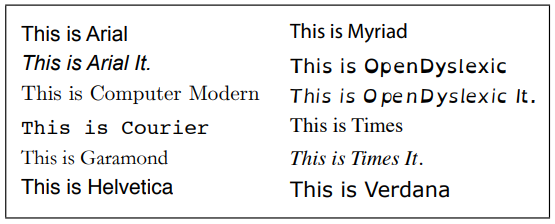
\includegraphics{figures/RolloFonts.PNG}
\end{center}
\caption{Figure 1 of \cite{Rello2013} showing the fonts used in their experiment. \label{fig:RelloFonts}}
\end{figure}


An \href{https://www.dyslexicadvantage.org/the-best-fonts-for-dyslexia/
}{informal article on a similar comparison of fonts} showed Dyslexie scoring well, but note that the comparison is unfair because the default font size in the text samples using Dyslexie was larger than the other fonts, this aside it showed Arial and Comic Sans both scoring well. The only formal study I found to do a broad and objective comparison of many fonts was \cite{Rello2013}, who compared the 12 fonts shown in Figure~\ref{fig:RelloFonts} using eye-tracking data to compare reading speed and fixation duration. Fixation duration turned out to be the more important measure, as had been demonstrated previously, and using this they showed that italics fonts were more difficult to read, while in general sans serif and  monospaced fonts seemed to be easier to read, although Courier was the only monospaced font they tested. They found the best fonts were Helvetica, Courier, Arial, Verdana and Computer Modern (CMU) although they did not test Comic Sans.  

\begin{figure}
\begin{center}
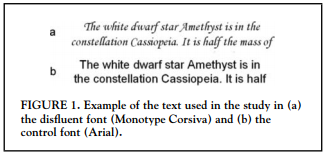
\includegraphics[scale=1.4]{figures/FrenchText.PNG}
\end{center}
\caption{Figure from \cite{French2013} showing example text samples. \label{fig:FrenchText}}
\end{figure}

On these issues the literature is divided at best, but there do seem to be some take home messages on how to make text easier to read in general, and in particular for dyslexic people:
\begin{itemize}
	\item {\huge Use a larger font size.}
	\item Do not use italics. If you need to emphasise some text, use \textbf{bold}.
	\item Use generous spacing settings, increase line spacing.
	\item Use a sans serif font, such as Arial, Comic Sans, Sans-serif Computer Modern, Verdana, or Helvetica. If for some reason you have to use a serif font, use one like Courier.
\end{itemize}

To throw a wrench in all the works (or maybe just play devil's advocate), \cite{French2013} demonstrates that easier to read fonts are less likely to result in comprehension, while using disfluent (difficult to read) fonts such as Monotype Corsiva causes more cognitive processing which results in better understanding of the underlying material. Ultimately, it is a complicated and not fully understood area, but there is some evidence to say that using a clear font can help some dyslexic people with reading, so given the ease of implementing such a change it is worth doing so.



\section*{Use of Colour}

Many people report that use of a coloured overlay or lenses to reduce visual stress can improve their reading. Again, similar to font --- the appeal is obvious, providing coloured overlays is very easy to do, the question is effectiveness. First of all, it is well accepted in the literature that this approach does not work for everyone, and for those that it does work, a different colour is required for each individual \cite{Lightstone1999}. There are two predominant approaches to determining the colour for an individual: use of \href{https://www.thedyslexiashop.co.uk/i-o-o-intuitive-coloured-a4-overlays.html}{I.O.O Intuitive Overlays} which offer 10 base colours and many more with pairwise combinations, or use of a \href{https://www.cerium.com.au/cerium-optical-technologies/intuitive-colorimeter}{Intuitive Colorimeter}, often used to determine lens colour. These are actually techniques originating from research into a condition called visual stress, also known as “Mears-Irlen” syndrome, and the evidence for the effectiveness of coloured overlays and lenses in reducing visual stress was very comprehensive in the 90s \cite{Jeanes1997}. In the double-blinded study \cite{Wilkins1994} they demonstrate that by manipulating an intuitive colorimeter to hold luminance constant and vary hue and chroma they can show that not only hue is important for reducing visual stress symptoms of eye-strain and headaches, but chromaticity is important too. Since the 90s interaction effects have been investigated between visual stress and dyslexia \cite{Singleton2005} as well as autism \cite{Ludlow2006}. Although the link between these conditions remains unclear: \cite{Singleton2005} claims to demonstrate that dyslexic people benefit from coloured overlays more than non-dyslexic people, while \cite{Henderson2013} claims to demonstrate that coloured overlays improve reading speed of jumbled text equally for dyslexic and non-dyslexic people. More concerning, \cite{Henderson2013}
also claims that in comparison, coloured overlays have no significant effect on reading speed or comprehension for either dyslexics or non-dyslexics when applied to connected (as opposed to jumbled) text, particularly concerning as much of the other research is done using jumbled text to estimate reading speed.

%Three studies (Jeans1997): 
%
%1. 50\% of students reported benefits to using a coloured overlay. Three months later the children tended to choose similar colours to what they chose the first time. 10 months later 20\% where still using the coloured overlays, but not the children who stopped using the coloured overlaps, demonstrated increased reading speed of jumbled words using the overlay compared with not using it. 
%
%2. children who used overlays (seperate group) compared their reading speed using a clear or gray overlay and had similar speeds, which where slower than using the coloured overlay --- indicating it was not just a matter of contrast. 
%
%3. In a third independant study, the increase in reading speed initially using the overlay successfully predicted the children that would still be using the overlay in the following 8 weeks.



\section*{Portioning Content / Timing}

This should go without saying as it is the essence of good teaching practice, but it is so important I thought it deserved to be emphasised with it's own section. 
\begin{itemize}
	\item Be clear in your instruction.
	\item Give bite sized steps.
	\item Give enough time for students to complete each step before giving the next step.
	\item Provide the steps in writing as well as verbally, so they can be referred back too.
	\item Don't rely only of verbal or only on written content, use both.
\end{itemize}
When reading through material suggesting strategies for accommodating dyslexic students, these and similar things just kept coming up and to me it just seems like... good teaching practice. All students should benefit from the above.



\section*{Tailoring Content through Formative Assessment}

Differentiation is important. What works for one student is not going to work for all students, and at the end of the day the essential key to successful outcomes with any given students is to learn and provide what those particular students need. As teachers we can access what our students need in various ways. Parents/ Guardians can be valuable resources. If you have students with reading/ writing difficulties, it is very likely they have been dealing with them for a long time, and they might just be able to tell you what works for them and what does not.

Formative assessments can help you identify students that might need special supports, but also allow you to tailor your content for the entire class. I like the idea of just doing something as easy as a 60 second activity similar to that proposed in \href{https://educationtechnologysolutions.com.au/2015/02/10-achievable-strategies-to-tackle-dyslexia-in-your-classroom-and-school/}{this article} where you photocopy some text onto a few different pieces of paper, or on white and hand out a bunch of coloured overlays, and ask your students which are easier to read. Explain why they might help, and offer to let the students keep the overlays. You could do a similar thing with a few different fonts and spacing settings in your text editor. It would take 5 minutes to set up, and could potentially improve the accessibility of your class dramatically. Beyond this, even if you do not subscribe to the results of  \cite{French2013}, or those of \cite{Henderson2013}, they still raise an important point: most of the research surrounding dyslexia is based around reading speed and measures of discomfort, and not comprehension. Although these things are important, particularly minimising any discomfort felt by our students, through formative assessment we can also check for comprehension and ensure that any strategies we are implementing are actually working to allow the students understand and learn. That is, after all, the goal (some might claim).

Finally, a personal reflection: I left differentiation for last because it is the most difficult to implement in practice, to no small degree due to the time constraints on us as teachers. But I also wanted to end on it, because in my view it is the most important. It also resonates the most strongly with my beliefs and values as a teacher: that each student is an individual, with their own strengths, and that successful teaching (to me) is building relationships with each individual student, learning their needs, their dreams, their strengths, and catering for them. It's hard work, but it's worth it.

\section*{References}

What follows is a list of less formal sources used when researching this topic that where not explicitly cited above. For the formal articles cited above, see the bibliography.
\begin{itemize}
	\item \href{https://www.dyslexia.com/about-dyslexia/understanding-dyslexia/guide-for-classroom-teachers/
}{A Dyslexic Child in the Classroom --- A Guide for Teachers and Parents (Patricia Hodge)},
	\item \href{https://www.theguardian.com/teacher-network/teacher-blog/2013/sep/09/supporting-students-with-dyslexia-teachers-tips-pupils}{Supporting students with dyslexia: tips, tricks and tech for teachers (David Imrie)},
	\item \href{https://educationtechnologysolutions.com.au/2015/02/10-achievable-strategies-to-tackle-dyslexia-in-your-classroom-and-school/}{10 Achievable Strategies to Tackle Dyslexia in Your Classroom and School (Michael Guy Clark)},
	\item \href{https://www.dyslexia-international.org/ONL/EN/Course/Welcome.htm
}{Dyslexia International Online Course},
	\item \href{https://blog.capterra.com/teaching-students-with-dyslexia-4-effective-lesson-plans/
}{Teaching Students with Dyslexia: 4 Effective Lesson Plans (Nick Morpus)},
	\item \href{https://www.britishcouncil.org/voices-magazine/how-teachers-can-help-learners-dyslexia
}{How teachers can help learners with dyslexia (Bríd Ní Chatháin)},
	\item \href{https://www.drgavinreid.com/free-resources/dyslexia-teaching-approaches/
}{Dyslexia: Teaching Approaches (Dr. Gavin Reid)},
	\item \href{http://www.dyslexiavictoriaonline.com/how-teachers-can-accommodate-the-dyslexic-student/
}{How Teachers Can Accommodate The Dyslexic Student (Dyslexia Victoria)}.
	\item \href{https://blog.dyslexia.com/evidence-based-but-does-it-work/}{“Evidence Based” — But does it work? (Abigail Marshall)}
\end{itemize}

\bibliographystyle{abbrv}
\bibliography{citations} 

\end{document}


